\documentclass[12pt,a4paper,svgnames]{article}
\usepackage[utf8]{inputenc}
\usepackage[T1]{fontenc}
\usepackage{amsmath}
\usepackage{amsfonts}
\usepackage{amssymb}
\usepackage{graphicx}
\usepackage[spanish,es-nodecimaldot,es-lcroman,es-tabla,es-noshorthands]{babel}
\usepackage[left=3cm,right=2cm, bottom=4cm]{geometry}
\usepackage{subfigure}
\usepackage{tikz}
\usepackage{xstring}
\usepackage{./tikz-uml}

%\setsansfont[Ligatures=TeX]{texgyreadventor}
%\setmainfont[Ligatures=TeX]{texgyrepagella}

%*******************************************************
%                 NO MODIFICAR
\newcommand*{\FSfont}[1]{%
  \fontencoding{T1}\fontfamily{#1}\selectfont}

\newlength{\tpheight}\setlength{\tpheight}{0.9\textheight}
\newlength{\txtheight}\setlength{\txtheight}{0.9\tpheight}
\newlength{\tpwidth}\setlength{\tpwidth}{0.9\textwidth}
\newlength{\txtwidth}\setlength{\txtwidth}{0.9\tpwidth}
\newlength{\drop}
%*******************************************************

% Crea una portada con los siguientes parámetros
%
% #1 : Título 
% #2 : Subtítulo
% #3 : Subsubtítulo
% #4 : Autor(es)
% #5 : Lugar
%

\newcommand*{\portada}[5]{
\begin{titlepage}
\begingroup
\vspace*{1cm}
\drop = 0.2\txtheight
\centering
\vfill
{\Huge \scshape #1}\\[\baselineskip]
{\Large \textbf{#2}}\\[\baselineskip]
{\Large \scshape #3}\\[\baselineskip]
\vspace*{0.3cm}
{\large \textit{#4}}\\[0.5\drop]

\includegraphics[scale=0.35]{./imagenes/logoURJC.jpg}
\vspace*{1.5cm}

{\large \scshape #5, \today} \par
\begin{center}
\end{center}
\vfill\null
\endgroup
\end{titlepage}
}
 %*****************************************************
 

\newcommand{\anadirproductoadministrador}{
\begin{tikzpicture}
\tikzumlset{fill state=white}
\umlstateinitial[name=initial]
\begin{umlstate}[x=0, y=-3,name=datos]{Iniciar sesión}
\end{umlstate}

\umlstatedecision[y=-5, name=permiso] 

\begin{umlstate}[x=0, y=-8,name=comprobar]{Añadir nuevo producto}
\end{umlstate}

\begin{umlstate}[y=-11,name=sesion]{Rellenar datos del producto}
\end{umlstate}

\begin{umlstate}[y=-14,name=actualizar]{Confirmar nuevo producto}
\end{umlstate}

\umlstatefinal[y=-16, name=final]

\umltrans{initial}{datos}
\umltrans{datos}{permiso}
\umltrans[arg1=correcto]{permiso}{comprobar}
\umltrans{comprobar}{sesion}
\umltrans{sesion}{actualizar}
\umltrans{actualizar}{final}
\umlHVHtrans[arg1=incorrecto, arm2=-4]{permiso}{datos}

\end{tikzpicture}
}

\newcommand{\comprarproducto}{
	\begin{tikzpicture}
	\tikzumlset{fill state=white}
	\umlstateinitial[name=initial]
	\begin{umlstate}[x=0, y=-3,name=datos]{Buscar producto}
	\end{umlstate}
	
	\umlstatedecision[y=-5, name=permiso] 
	
	\begin{umlstate}[x=0, y=-8,name=comprobar]{Añadir prodcuto al carrito}
	\end{umlstate}
	
	\begin{umlstate}[y=-11,name=sesion]{Ver cesta}
	\end{umlstate}
	
	\begin{umlstate}[y=-14,name=actualizar]{Realizar pedido}
	\end{umlstate}
	
	\umlstatefinal[y=-16, name=final]
	
	\umltrans{initial}{datos}
	\umltrans{datos}{permiso}
	\umltrans[arg1=encontrado]{permiso}{comprobar}
	\umltrans{comprobar}{sesion}
	\umltrans{sesion}{actualizar}
	\umltrans{actualizar}{final}
	\umlHVHtrans[arg1=no encontrado, arm2=-4]{permiso}{final}
	
	\end{tikzpicture}
}

\newcommand{\casosdeuso}{
	\begin{tikzpicture}
	\tikzumlset{fill usecase=white}
	\tikzumlset{fill note=gray!30}
	\tikzumlset{font=\tiny}
	
	\umlactor[x=0, y=3]{USUARIO}
	\umlactor[x=0, y=-2]{ADMIN}
	
	\umlusecase[x=3, y=4, name=buscarproductos]{Buscar productos}
	\umlusecase[x=3, y=2, name=realizarpedido]{Realizar pedido}
	\umlusecase[x=8, y=3, name=anadirproductocarro]{Añadir producto producto al carro}
	\umlusecase[x=8, y=2, name=vercarro]{Ver carro}
	
	\umlassoc{USUARIO}{realizarpedido}
	\umlassoc{USUARIO}{buscarproductos}
	
	
	\umlinclude{realizarpedido}{anadirproductocarro}
	\umlinclude{realizarpedido}{vercarro}
	
	
	\umlusecase[x=3, y=-1, name=anadirproducto]{Añadir productos}
	\umlusecase[x=3, y=-2, name=verproductos]{Ver productos}
	\umlusecase[x=3, y=-3, name=verpedido]{Ver pedido}

	\umlusecase[x=7, y=-2, name=modificarproducto]{Modificar producto}
	\umlusecase[x=7, y=-3, name=borrarproductos]{Borrar productos}
	\umlusecase[x=7, y=-4, name=borrarpedido]{Borrar pedido}
	\umlusecase[x=7, y=-5, name=actualizarestadopedido]{Actualizar estado pedido}
	
	\umlusecase[x=11, y=-2, name=iniciarsesion]{Iniciar sesión}
	
	\umlassoc{ADMIN}{anadirproducto}
	\umlassoc{ADMIN}{verproductos}
	\umlassoc{ADMIN}{verpedido}
	
	
	
	\umlinclude{anadirproducto}{iniciarsesion}
	\umlextend{modificarproducto}{verproductos}
	\umlextend{borrarproductos}{verproductos}
	\umlextend{borrarpedido}{verpedido}
	\umlextend{actualizarestadopedido}{verpedido}
	\umlextend{realizarpedido}{vercarro}
	
	\umlinclude{modificarproducto}{iniciarsesion}
	\umlinclude{borrarproductos}{iniciarsesion}
	\umlinclude{borrarpedido}{iniciarsesion}
	\umlinclude{actualizarestadopedido}{iniciarsesion}
	
	
	\end{tikzpicture}
}

\newcommand{\clases}{
	
\begin{tikzpicture}
	

\umlclass[x=0, y=0]{AlmostCart}{
}{
}

\umlclass[x=5, y=0]{Cart}{
}{
}

\umlclass[x=0, y=-5]{Product}{
}{
}

\umlclass[x=5, y=-5]{Order}{
}{
}

% Relaciones

\umlcompo[mult2=1..n]{Cart}{AlmostCart}

\umlcompo[mult2=1..n]{Order}{Cart}

\umlassoc[mult2=1, mult1=1..n]{AlmostCart}{Product}


\end{tikzpicture}

}


\newcommand*{\autores}{
\begin{tabular}{r l}
GII+GIS: & Germán Alonso Azcutia \\
GIS+MAT: & José Ignacio Escribano Pablos
\end{tabular}
}

\begin{document}

\pagenumbering{alph}
\setcounter{page}{1}

\portada{Práctica 1}{Diseño de Aplicaciones Web}{Implementación de una tienda virtual}{\autores}{Móstoles}

\tableofcontents
\thispagestyle{empty}
\newpage

\pagenumbering{arabic}
\setcounter{page}{1}


\section{Introducción}
Para la realización de la práctica vamos a usar el patrón de arquitectura de software \\
\texttt{Modelo-Vista-Controlador(MVC)}, que como su propio nombre indica, define la organización independiente del Modelo (información y lógica de negocio), la Vista (interfaz con el usuario) y el Controlador (intermediario entre modelo y vista).\\

\begin{figure}[htbp]
\centering
\subfigure{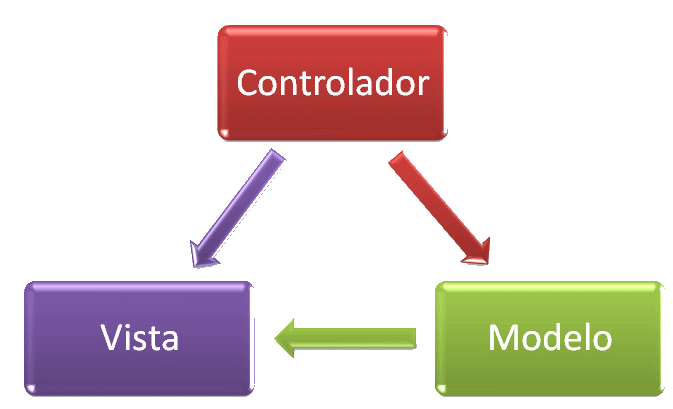
\includegraphics[width=65mm]{./imagenes/mvc}}
\caption{Patrón de arquitectura Modelo Vista Controlador (MVC)}
\end{figure}

Para llevar a cabo la explicación de la responsabilidad de cada clase, vamos a dividir dicha explicación en las tres partes del patrón.\\

Pero antes, veamos los diagramas \texttt{UML} de nuestra aplicación web.

\clearpage

\section{Diagramas UML}
\subsection{Diagrama de casos de uso}
 
El diagrama de casos de uso de la Figura~\ref{fig:casosdeuso} muestra que la aplicación tiene dos roles distintos dentro de la aplicación: usuario y administrador. El primero de ellos puede ver productos, añadirlos al carrito, ver su carro, y el segundo puede añadir productos al catálogo de la tienda, modificarlos, ver los pedidos, así como todas las acciones derivadas de las anteriores.\\

Esto supone que hay que distinguir casos distintos casos, ya sea para un usuario o para el administrador.  
\begin{figure}[htbp]
	\centering
	\casosdeuso
	\caption{Diagrama de casos de uso de la aplicación}
	\label{fig:casosdeuso}
\end{figure}

\clearpage

\subsection{Diagrama de clases}

El diagrama de clases muestra todas las clases que manejarán la lógica de la aplicación. Estas clases son ProductWithCuantity, Cart, Product y Order. La descripción de cada clase se puede ver en la Sección~\ref{sec:descripcion}.

\begin{figure}[htbp] 
	\centering
	\clases
	\caption{Diagrama de clases de la aplicación}
\end{figure}

\subsection{Diagramas de actividad}

Como hemos comentado anteriormente, debemos distinguir tareas para un usuario normal y el administrador. Esto se refleja en los diagramas de actividad: en el caso de un usuario normal no es necesario iniciar sesión (en el enunciado de la práctica se especifica que no hay usuarios, salvo el administrador), mientras que en el adminstrador sí que es necesario.\\

Un ejemplo de lo anterior se puede ver en las Figuras~\ref{fig:actividad1}~y~\ref{fig:actividad2} donde no es necesario iniciar sesión para comprar un producto de la tienda, y, por el contrario, sí que lo es para añadir un producto al catálogo de la tienda.  

\begin{figure}[htbp] 
	\centering
	\comprarproducto
	\caption{Diagrama de secuencia de comprar producto}
	\label{fig:actividad1}
\end{figure}

\begin{figure}[htbp]
	\centering
	\anadirproductoadministrador
	\caption{Diagrama de secuencia de añadir producto como administrador}
	\label{fig:actividad2}
\end{figure}

\clearpage

\section{Descripción de las clases}\label{sec:descripcion}
\subsection{Modelo}
\subsubsection{Clase Product}
Esta clase define el objeto producto y las propiedades y métodos de los que dispondrán los productos de nuestra web.\\
\subsubsection{Clase ProductWithCuantity}
La clase \texttt{ProductWithCuantity} define un producto que estará en el carro de compra y la cantidad de dicho producto almacenada en el carro. Por tanto, se compone de un producto y su cantidad.\\
\subsubsection{Clase Cart}
Esta clase define el carro de compra de cada usuario. Está compuesto por un ArrayList de \texttt{ProductWithCuantity} (que serán el total de productos en la cesta) y el precio total del carro.\\
\subsubsection{Clase Order}
La clase \texttt{Order} define el pedido del usuario, es decir, la confirmación de querer comprar su carro de compra. Por ello, esta clase contiene un atributo carro, además del estado del pedido (pendiente o preparado) y los datos correspondientes del usuario que ha realizado el pedido.\\
\subsubsection{Interfaz ProductRepository}
Es una clase que extiende de CrudRepository, interfaz genérica que ofrece operaciones tipo CRUD (Create-Read-Update-Delete) para acceder a los datos de la base de datos. Nosotros lo utilizaremos en esta clase para realizar consultas sobre los productos en la BD.\\
\subsubsection{Interfaz OrdertRepository}
Al igual que \texttt{ProductRepository}, esta clase extiende de CrudRepository, pero esta vez la clase nos servirá para realizar consultas a la BD sobre los pedidos.\\
\subsection{Controlador}
\subsubsection{Clase ProductController}
Esta clase es el controlador de nuestra aplicación, es decir, responderá a los eventos de las diferentes vistas (mayoritariamente acciones del usuario, como pulsar un botón) y hará peticiones al modelo cuando se hace alguna solicitud sobre la información.
Un ejemplo podría ser cuando el usuario pulsa sobre la categoría "Videoconsolas", la clase \texttt{ProductController} responderá al evento buscando en la base de datos los productos pertenecientes a dicha categoría y devolviendo una vista donde aparezcan estos productos.\\
\subsection{Vista}
\subsubsection{index.html}
Esta vista corresponde a la página principal de nuestra aplicación web.
\subsubsection{product.html}
En \texttt{product.html} encontramos la vista donde se ve un producto seleccionado (botón más información), con la información completa de dicho producto y la posibilidad de añadirlo al carro.
\subsubsection{cart.html}
En esta vista tenemos nuestro carro de compra, donde podremos aumentar o disminuir la cantidad de los productos que se encuentren en la cesta, eliminarlos y realizar el pedido.
\subsubsection{admin.html}
Esta vista es la pantalla principal del administrador, en ella aparecen los distintos productos de la web, donde tenemos las opciones de añadir nuevos productos, borrar o editar productos existentes, filtrar los productos o ver los pedidos.
\subsubsection{new.html}
En esta vista tenemos un formulario que nos permitirá añadir nuevos productos a la tienda.
\subsubsection{edit.html}
En esta vista tenemos un formulario que nos permitirá editar los productos de la tienda.
\subsubsection{order.html}
Esta vista es otro formulario en donde se pedirán los datos al usuario para realizar el pedido.
\subsubsection{orders.html}
En \texttt{orders.html} se mostrarán los distintos pedidos de la tienda donde tendremos la opción de cambiar su estado (pendiente o preparado). Además, se podrán filtrar los pedidos mediante su estado, nombre o fecha.

\clearpage

\section{Recorrido por la aplicación}

\end{document}
